\documentclass[10pt]{article}

\usepackage[paperwidth=29.5cm,paperheight=11.1cm,margin=0cm,noheadfoot]{geometry}
\usepackage{graphicx}
\usepackage[utf8]{inputenc}
\usepackage{parskip}
\usepackage{array}
\usepackage{multicol}
\usepackage{xcolor}
\usepackage{titlesec}
\usepackage{pdfpages}
\usepackage[ngerman]{babel}
\usepackage{csquotes}
\pagestyle{empty}

% Left-aligned section headings with a size between \large and \Large.
\titleformat{\section}[block]{\normalfont\bfseries\fontsize{13}{15}\selectfont\raggedright}{}{0pt}{}
% Compact spacing for month headings.
\titlespacing*{\section}{0pt}{0.35em}{0.2em}

% 4 A7 panels per page (29.7cm / 4 = 7.425cm)
\newlength{\panelwidth}
\setlength{\panelwidth}{0.25\paperwidth}
\newlength{\panelmargintop}
\newlength{\panelmarginbottom}
\newlength{\panelmarginx}
\newlength{\panelheight}
\setlength{\panelmargintop}{5mm}
\setlength{\panelmarginbottom}{6mm}
\setlength{\panelmarginx}{7mm}
\setlength{\panelheight}{\dimexpr\textheight-8pt\relax}

% A panel with consistent inner margins on all sides.
\newenvironment{panel}{%
\begin{minipage}[t][\panelheight][t]{\panelwidth}%
\vspace*{\panelmargintop}%
\hspace*{\panelmarginx}%
\begin{minipage}[t][\dimexpr\panelheight-\panelmargintop-\panelmarginbottom\relax][t]{\dimexpr\panelwidth-2\panelmarginx\relax}%
}{%
\end{minipage}%
\end{minipage}%
}

% A group of adjacent panels (e.g. 3x A7) with one shared text flow area.
\newenvironment{panelgroup}[1]{%
\begin{minipage}[t][\panelheight][t]{\dimexpr #1\panelwidth\relax}%
\vspace*{\panelmargintop}%
\hspace*{\panelmarginx}%
\begin{minipage}[t][\dimexpr\panelheight-\panelmargintop-\panelmarginbottom\relax][t]{\dimexpr #1\panelwidth-2\panelmarginx\relax}%
}{%
\end{minipage}%
\end{minipage}%
}

\newcommand{\tinyscript}{\fontsize{6}{7}\selectfont}

% Event/contact helpers for automatic vertical spacing in fixed-height panels.
\newcommand{\eventitem}[2]{%
\par\noindent
\parbox[t]{\linewidth}{%
\begin{tabular}{@{}>{\raggedright\arraybackslash}p{0.29\linewidth}@{\hspace{0.5em}}>{\raggedright\arraybackslash}p{\dimexpr0.71\linewidth-0.5em\relax}@{}}
\textbf{#1} & #2
\end{tabular}
}%
\par\vspace{0.6em}
}
% Helpers for multiple points under one date (e.g. multiple times).
\newcommand{\eventpoints}[1]{\begin{tabular}[t]{@{}l@{}}#1\end{tabular}}
\newcommand{\eventpoint}[1]{#1}
\newcommand{\eventmeta}[1]{\mbox{(#1)}}

\begin{document}
\small
\setlength{\parskip}{0pt}
\setlength{\parindent}{0pt}

%%%%%%%%%%%%%%%%%%%%%%%%%%%%%%%%%%%%%%%%%%%%%%%%%%%%
% PAGE 1 (OUTSIDE)
%%%%%%%%%%%%%%%%%%%%%%%%%%%%%%%%%%%%%%%%%%%%%%%%%%%%

\noindent
\makebox[\paperwidth][l]{%

\begin{panel}
\section*{Über Burggraf}

der katholische Studentenverein Burggraf
ist ein nichtschlagender und farbenführender
Studentenverein im Kartellverband
katholischer deutscher Studentenvereine (KV).
\\\\
Über unseren Dachverband bilden wir ein
deutschlandweites Netzwerk von Akademikern aller Fakultäten.
Wie der KV haben wir uns den Prinzipien
Religion, Wissenschaft und Freundschaft
verschrieben. Das Hochhalten und Wahren dieser 
Prinzipien sowie des studentischen Brauchtums
ist der Kern unseres Lebensbundes.
\\\\
Hierzu organisiert die Aktivitas jedes Semester ein Semesterprogramm mit den
verschiedensten Veranstaltungen von
wissenschaftlichen Vorträgen über traditionelle Kneipen bis hin zu gemeinsamen
Aktivenfahrten mit Wanderungen in den
Bergen.

\includepdf[pages=1]{pdfs/overlay_band.pdf}
\end{panel}%
\begin{panel}
\section*{Allgemeines und Erklärungen}

\textbf{Veranstaltungen}

\begin{tabular}{ll}
ho & hochoffiziell \\
o  & offiziell \\
io & inoffiziell \\
\end{tabular}

\vspace{1em}

\textbf{Zeitangaben}

{\scriptsize
\begin{tabular}{ll}
st  & sine tempore (pünktlich) \\
ct  & cum tempore (Viertel nach) \\
mct & magno cum tempore (Halb nach) \\
mmct & maximo cum tempore (Dreiviertel nach) \\
\end{tabular}
}
\vspace{1em}

\textbf{Stammtische bei Burggraf} \\
Jeden zweiten Montag im Monat trifft sich
die Aktivitas gemeinsam abwechselnd zum
Stiefelmontag auf dem Haus 
oder zum Bowlingstammtisch beim Blu Bowl 
in der Zeltnerstraße 19, 90443 Nürnberg.
\\\\
Jeden vierten Montag im Monat findet im
Anschluss an die Convente um 20\,h ct ein
Stammtisch der Aktivitas auf dem Haus
statt.

\end{panel}%
\begin{panel}
\section*{Vorstand der Verbindung}
\vspace{0.4em}

{\tinyscript
\begin{tabular}{@{}p{0.48\linewidth}p{0.48\linewidth}@{}}
\parbox[t]{\linewidth}{%
{\small\textbf{x}}\\
David Spies\\
stud. inf.\\
senior@kstv-\\burggraf.de
}
&
\parbox[t]{\linewidth}{%
{\small\textbf{vx}}\\
Marc Kupp\\
stud. ing.\\
consenior@kstv-burggraf.de
}\\[0.8em]
\\
\parbox[t]{\linewidth}{%
{\small\textbf{FM}}\\
Felix Troßmann\\
stud. soz. arb.\\
fuxmajor@kstv-burggraf.de
}
&
\parbox[t]{\linewidth}{%
{\small\textbf{xx}}\\
Maximilian Birke\\
cand. iur.\\
scriptor@kstv-burggraf.de
}\\[0.8em]
\\
\parbox[t]{\linewidth}{%
{\small\textbf{xxx}}\\
Rocco Hauboldt\\
stud. inf.\\
quaestor@kstv-burggraf.de
}

\end{tabular}

\vspace{3em}

\vspace{0.3em}
\textbf{Philistersenior:}\\
Dipl.-Kfm. Harald Litzka\\
E-mail: harald.litzka@kstv-burggraf.de

\vspace{0.3em}
\textbf{Studienfördervereinsvorsitzender:}\\
B.Sc. Inf. Christoph Euskirchen\\
E-mail: christoph.euskirchen@kstv-burggraf.de

\vspace{0.3em}
\textbf{Ehrenphilistersenior:}\\
Dipl.-Kfm. Ludwig Weihmann\\
E-mail: ludwig.weihmann@kstv-burggraf.de

\vspace{0.3em}
\textbf{Ortszirkel \enquote{Nürnberger Trichter}}\\
Prof. Dr. Heinz Tröster\\
E-mail: heinz.troester@kstv-burggraf.de


}



\end{panel}%
\begin{panel}
\begin{center}

\vspace{0.75cm}

{\Large K.St.V.}\\
{\LARGE \textbf{Burggraf}}\\
im KV zu Nürnberg


\includegraphics[width=\linewidth]{figures/wappen.png}

{\large Sommersemester 2026}

\end{center}
\end{panel}%
}%

%%%%%%%%%%%%%%%%%%%%%%%%%%%%%%%%%%%%%%%%%%%%%%%%%%%%
% PAGE 2 (INSIDE)
%%%%%%%%%%%%%%%%%%%%%%%%%%%%%%%%%%%%%%%%%%%%%%%%%%%%
%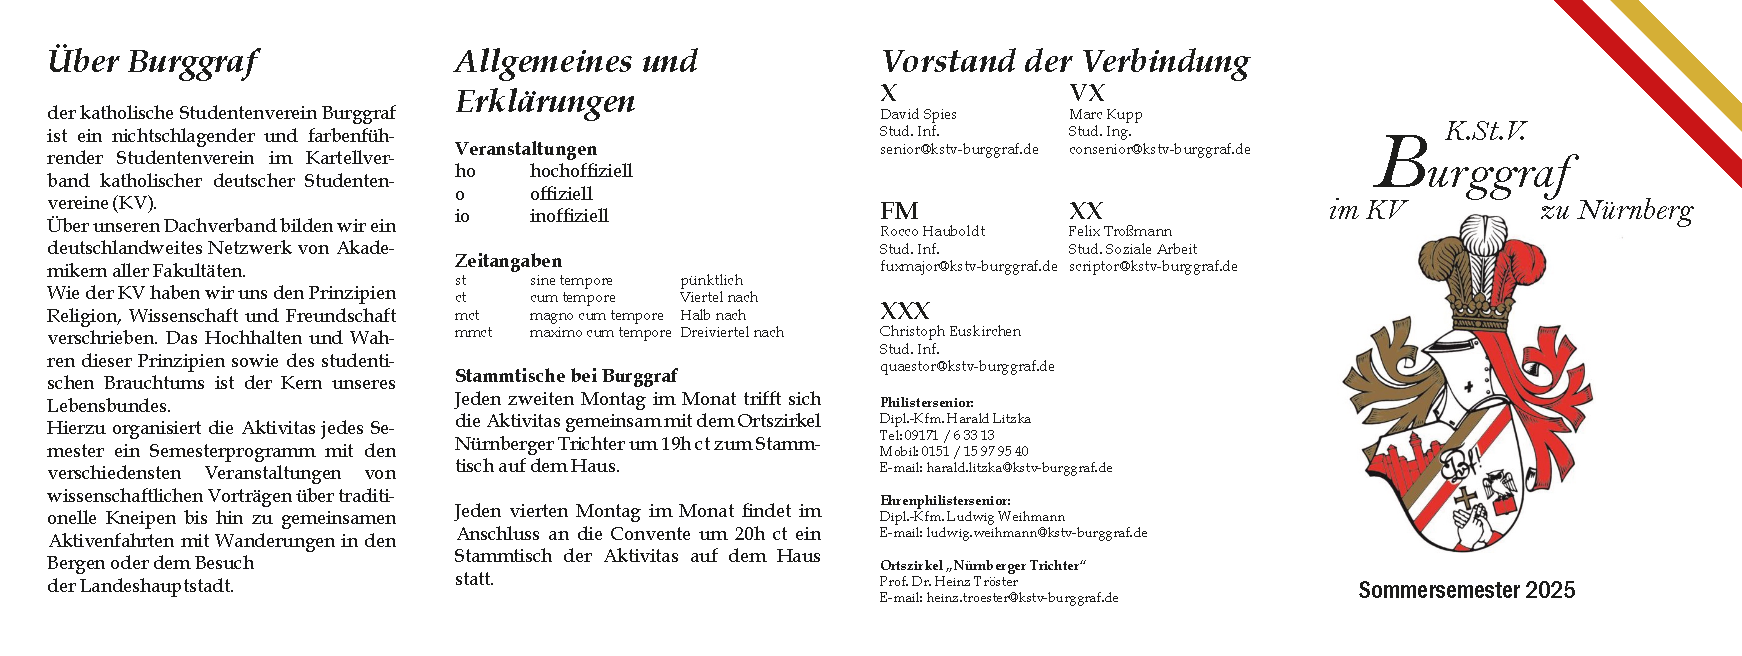
\includepdf[pages=1]{old/SS2025.pdf}
\clearpage
\noindent

\makebox[\paperwidth][l]{%
\begin{panelgroup}{4}

% Match page 1 panel spacing: each column keeps left/right inner margins,
% so the visual gap between adjacent text areas is 2*\panelmarginx.
\setlength{\columnsep}{\dimexpr2\panelmarginx\relax}
\setlength{\multicolsep}{0pt}
\begin{multicols}{4}
\raggedcolumns


Liebe Farben-, Kartell- und Bundesbrüder,\
verehrte Damen, Gäste und Freunde,\ 
\\\\
die Aktivitas des K.St.V. Burggraf im KV zu Nürnberg erlaubt sich,
Ihnen und euch das Programm für das Sommersemester 2026 zu
überreichen und lädt damit höflichst zur Teilnahme an den
Veranstaltungen, insbesondere den Stammtischen jeden zweiten und
vierten Montag im Monat, ein.
\\\\
Für das kommende Semester wünschen wir allen Gesundheit und viel
Erfolg in Beruf, Studium und Privatleben.

\vspace{0.6em}
\noindent
{\scriptsize
\begin{minipage}[t]{0.42\linewidth}
Für die Aktivitas:\\\\
{\normalsize\textbf{David Spies}}\\
Stud. Inf.\\
Aktivensenior
\end{minipage}\hfill
\begin{minipage}[t]{0.52\linewidth}
Für die Altherrenschaft:\\\\
{\normalsize\textbf{Harald Litzka}}\\
Dipl.-Kaufmann\\
Altherrensenior
\end{minipage}

\vspace{1em}

\section*{März}
\eventitem{Mo 16.03.}{\eventpoints{%
\eventpoint{AC/BC \eventmeta{19\,h ct / ho} adH}\\
\eventpoint{Stammtisch \eventmeta{20\,h ct / io} adH}%
}}
\eventitem{Mo 23.03.}{Bowlingstammtisch \eventmeta{18\,h mmct / io} Blu Bowl}
\eventitem{Sa 28.03.}{Ankneipe \eventmeta{19\,h ct / ho} adH}
\eventitem{So 29.03.}{Semersterantrittsgottesdienst \eventmeta{9\,h mct / ho} Kirche St. Elisabeth}
\eventitem{Mo 30.03.}{\eventpoints{%
\eventpoint{AC/BC \eventmeta{19\,h ct / ho} adH}\\
\eventpoint{Stammtisch \eventmeta{20\,h ct / io} adH}%
}}

\section*{April}
\eventitem{Sa 11.04.}{Säubern der Stolpersteine in Nürnberg \eventmeta{14\,h ct / o} adH}
\eventitem{Mo 13.04.}{\eventpoints{%
\eventpoint{AC/BC \eventmeta{19\,h ct / ho} adH}\\
\eventpoint{Stammtisch \eventmeta{20\,h ct / io} adH}%
}}
\eventitem{Mo 20.04.}{Stiefelmontag \eventmeta{19\,h ct / io} adH}
\eventitem{Mo 27.04.}{\eventpoints{%
\eventpoint{AC/BC \eventmeta{19\,h ct / ho} adH}\\
\eventpoint{Stammtisch \eventmeta{20\,h ct / io} adH}%
}}

\section*{Mai}
\eventitem{Mo 04.05.}{Bowlingstammtisch \eventmeta{18\,h mmct / io} Blu Bowl}
\eventitem{Fr 08.05.}{Begrüßungsabend Stiftungsfest \eventmeta{19\,h ct / ho} adH}
\eventitem{Sa 09.05.}{Stiftungsfestkommers \eventmeta{19\,h ct / ho} Pfründnerstraße 20, Nürnberg}
\eventitem{So 10.05.}{Gottesdienst zum Stiftungsfest \eventmeta{11\,h mct / ho} Kirche St. Elisabeth}

\section*{Juni}
\eventitem{Mo 01.06.}{Bowlingstammtisch \eventmeta{18\,h mmct / io} Blu Bowl}
\eventitem{Mo 08.06.}{\eventpoints{%
\eventpoint{AC/BC \eventmeta{19\,h ct / ho} adH}\\
\eventpoint{Stammtisch \eventmeta{20\,h ct / io} adH}%
}}
\eventitem{Mo 15.06.}{Stiefelmontag \eventmeta{19\,h ct / io} adH}
\eventitem{Mo 22.06.}{\eventpoints{%
\eventpoint{AC/BC \eventmeta{19\,h ct / ho} adH}\\
\eventpoint{Stammtisch \eventmeta{20\,h ct / io} adH}%
}}
\eventitem{Sa 27.06.}{Ex-adH in loco bummeln \eventmeta{16\,h ct / ho} adH}
\eventitem{Mo 29.06.}{Bowlingstammtisch \eventmeta{18\,h mmct / io} Blu Bowl}

\section*{Juli}
\eventitem{Sa 04.07.}{Schlauchboot fahren auf dem Wöhrder See \eventmeta{13\,h ct adH / io}}
\eventitem{Mo 06.07.}{\eventpoints{%
\eventpoint{AC/BC \eventmeta{19\,h ct / ho} adH}\\
\eventpoint{Stammtisch \eventmeta{20\,h ct / io} adH}%
}}
\eventitem{Mo 13.07.}{Stiefelmontag \eventmeta{19\,h ct / io} adH}
% \eventitem{Mo 20.07.}{\eventpoints{%
% \eventpoint{AC/BC \eventmeta{19\,h ct / ho} adH}\\
% \eventpoint{Stammtisch \eventmeta{20\,h ct / io} adH}%
% }}
\eventitem{Mo 27.07.}{Bowlingstammtisch \eventmeta{18\,h mmct / io} Blu Bowl}
\eventitem{Fr 31.07.}{Exkneipe \eventmeta{19\,h ct / ho} adH}

\section*{August}
\eventitem{Sa 01.08.}{Sommerpoolparty \eventmeta{14\,h ct / io} Garten adH }
\eventitem{So 02.08.}{Semesterexgottesdienst \eventmeta{11\,h mct / ho} Kirche St. Elisabeth}
\eventitem{Mo 03.08.}{\eventpoints{%
\eventpoint{AC/BC/DC/WC \eventmeta{19\,h ct / ho} adH}\\
\eventpoint{Stammtisch \eventmeta{20\,h ct / io} adH}%
}}

}


\vspace*{\fill}


{\scriptsize
\textbf{Unser Haus}\\
Regensburger Straße 30\\
90478 Nürnberg

\vspace{0.35em}
\textbf{Bankverbindungen}\\
Aktivitas: VR Bank Metropolregion Nürnberg \quad \\IBAN: DE41 7606 9559 0002 6309 74\\[0.25em]
Altherrenverein: LIGA Bank Regensburg \quad \\IBAN: DE39 7509 0300 0005 1249 99\\[0.25em]
Studienförderverein: LIGA Bank Regensburg \quad \\IBAN: DE86 7509 0300 0005 1000 97

\vspace{0.5em}
\textbf{Kontakt}\\
\begin{tabular}{@{}p{0.26\linewidth}p{0.70\linewidth}@{}}
E-Mail: & siehe Vorstand der Verbindung\\
Tel: & 0911 / 46206632\\
Web: & kstv-burggraf.de\\
Instagram: & @kstv\_burggraf
\end{tabular}
}

% Optional: use \columnbreak to force a manual split point.
\end{multicols}

\end{panelgroup}%
}

%\includepdf[pages=2]{old/SS2025.pdf}

\end{document}